\label{4_investigatory_experiments}

\begin{comment}
INTRO: What will you look at in this chapter and why? Again, point back to the summary in the last chapter, and say that here you want to experiment with and evaluate the proposed “solution”.
\end{comment}

% INTRO:
\section{Intro}
\begin{comment}
    List of the different runs that have been made.
\end{comment}


In this chapter, the Alpaca-VQA model presented in the previous chapter is tested on two different dataset sizes. First, hyperparameters, their values, and the reasons for choosing these are discussed. Then an investigatory experiment will be conducted using a smaller dataset to get initial results for training on more data. 
These results will be analyzed to understand better how the model responds to the data, aiding understanding how the model responds to the data.
The Alpaca-VQA model is then trained on 20,000 samples, and its results are discussed. Methods for visualizing transition scores and training a proxy model explained by \gls{lime} are implemented when the Alpaca-VQA model has finished training. 
The insights from these supplementary methods uncovered a possibility that the model did not evaluate the image features when predicting an answer. A language-only Alpaca-VQA model was tested to test this hypothesis, and its findings are discussed. 
Finally, a more general examination of the findings in this work is discussed. 


\begin{comment}
MIDDLE SECTIONS: Explain your experiments and evaluations. Include a detailed description of the data you have used, and which metrics you include. It is nice to discuss what the results also mean (in general and in the context of your problem statement), not only what you can observe. Also, try to explain WHY the results turn out as they do. You are a researcher and should try to understand why things happen, not only observe what happens.
\end{comment}

\section{Hyperparameters}
    The Alpaca-VQA model is based on the Stanford Alpaca model and therefore draws inspiration when deciding on hyperparameters from their findings.
    To finetune the Stanford Alpaca model, the authors suggest training for two or three epochs. The low number of epochs is not to let the model forget the previous knowledge and still be able to use the knowledge gathered from the original training corpus, known as \textit{catastrophic forgetting}. Therefore, for the following experiments, the hyperparameters were chosen as in \autoref{table:hyperparameters_alpaca}. 
    
    The \gls{lora} parameters were selected to be the same as the original Alpaca-LoRA implementation. 
    The transformer architecture contains four weight matrices for the self-attention module. These weights are for \textit{query} ($W_q$), \textit{key} ($W_k$), \textit{value} ($W_v$) and \textit{output} ($W_o$).
    In the paper introducing \gls{lora}, the authors find that choosing to apply \gls{lora} to the attention weights for \glspl{llm}, specifically GPT-3 on the datasets WikiSQL \cite{zhongSeq2SQLGeneratingStructured2017} and MultiNLI \cite{williamsBroadCoverageChallengeCorpus2018}, they achieved the best results overall by only adapting the $W_q$ and $W_v$ matrices. The developer of Alpaca-LoRA also confirmed these results, and therefore the experiments in this thesis will also use these update matrices.
    The authors of \gls{lora} also did experiments for GPT-2 and GPT-3 to see which effect the rank \textit{r} would have on the performance. They found that \gls{lora} performs competitively with small values of \textit{r}, especially when only adapting $W_q$ and $W_v$.

    As seen in \autoref{table:lora_parms}, the \gls{lora} update parameters are only 0.0622\% of the original amount of trainable parameters in the Alpaca-VQA model. This low amount of trainable parameters using \gls{lora} update matrices results in considerably faster training and lower memory use.

    
    The rationale for deciding on the batch size and micro-batch size values was to make it fit in the available \gls{ram} on the \gls{gpu} it was trained on. Since the current state of the code can only utilize a single \gls{gpu}, it was necessary to fit the model on the \gls{gpu} while training. 
    The \glspl{gpu} used for this experiment was an Nvidia RTX2080Ti with 11 GB of \gls{vram} and an Nvidia A100 with 40 GB of \gls{vram}. For the initial experiment, the smaller RTX2080Ti was used not to demand more compute resources than needed. The A100 was used when training on the larger datasets, and the batch size was doubled to 256, which benefited from more \gls{vram}. The increased batch size would allow the model to see more of the samples simultaneously during training.
    The number of epochs was kept to three while the step length was increased, effectively making the model evaluate more often in each epoch.
    
    The size of the validation set was chosen to be roughly 30\% of the training data, and the cutoff length was chosen to be 1485, as this corresponds to $256 \text{ question tokens} + 1229 \text{ tokens from the encoded image}$, as discussed in Section \ref{sec:3_cutoff}. This token length should allow the model to see most of the available input data, both text and images when predicting the output.

    The temperature parameter influences the probabilities when predicting new tokens. In practice is a measure of how creative the language model should be during text generation. A lower temperature value makes the model choose tokens it is more confident are correct, and a larger value makes it more creative. As this task is to answer a question, the goal is more based on facts than creativity, and therefore the temperature was chosen to be 0.1.

    During generation, the Alpaca-VQA model uses beam search with four beams. This means that it generates and searches in four sequences before deciding on the sequence with the highest combined transition score. This sequence is the one that the model is most confident fulfills the task.
    The values of \textit{top-K} and \textit{top-p} influence how many words are considered in the probability distribution during token generation. A top-K of 40 means it considers the 40 most probable tokens in the distribution. Top-p narrows down this distribution of top-K words to the smallest group that fulfills a cumulative probability above the set value. 
    With these hyperparameters set during generation, the Alpaca-VQA model achieves a reasonable broad distribution of tokens to sample from while maintaining the computation demand reasonable. 
    
    If no further details are given in the experiments, the parameters described here are the ones used in the following experiments.

    \begin{table}[htb]
    \centering
    \begin{tabular}{ r r c } 
         \multicolumn{3}{c}{\textbf{Alpaca-VQA Hyperparameters}}\\
        \toprule
           \multicolumn{2}{c}{\textbf{Hyperparameter}} & \textbf{Value}\\ 
        \midrule
            \multicolumn{3}{c}{\textbf{Training}}\\
            
            \multicolumn{2}{r}{Batch size:} & 128 \\
            \multicolumn{2}{r}{Micro batch size:} & 4 \\
            \multicolumn{2}{r}{Number of epochs:}& 3 \\
            \multicolumn{2}{r}{Learning rate:} & 0.0003 \\ 
            \multicolumn{2}{r}{Validation set size:} & 30\% of training data\\
        \midrule
            \multicolumn{3}{c}{\textbf{Text Generation}}\\
            \multicolumn{2}{r}{Temperature:} & 0.1\\
             \multicolumn{2}{r}{Cutoff length:} & 1485 \\
            \multicolumn{2}{r}{Top-p:} & 0.75\\
            \multicolumn{2}{r}{Top-K:} & 40\\
            \multicolumn{2}{r}{Number of beams:} & 4\\
        \midrule
            \multicolumn{3}{c}{\textbf{LoRA}}\\
            \multicolumn{2}{r}{Rank r:} & 8 \\
            \multicolumn{2}{r}{Alpha $\alpha$:} & 16 \\
            \multicolumn{2}{r}{Dropout:} & 0.05 \\
            \multicolumn{2}{r}{Weight Matrices:} & $W_q$, $W_v$ \\[0.5ex]
        \bottomrule
    \end{tabular}
    \caption{Hyperparmaters selected for the initial experiment with Alpaca-VQA, fine-tuning the LoRA matrices on the ImageCLEFmed-MEDVQA-GI-2023 dataset.}
    \label{table:hyperparameters_alpaca}
    \end{table}

    \begin{table}[htb]
    \centering
    \begin{tabular}{ r c } 
        \multicolumn{2}{c}{\textbf{LoRA Training Parameters}}\\
        \toprule
             %[0.5ex] 
           Parameter & Value \\
        \midrule
            Number of trainable LoRA parameters: & 4,194,304\\
            All parameters in Alpaca-VQA: & 6,742,609,920\\
            Trainable percent: & 0.0622\%\\[0.5ex]
        \bottomrule
    \end{tabular}
    \caption{Overview of the number of trained parameters using LoRA.}
    \label{table:lora_parms}
    \end{table}

    In the next section, an investigatory experiment will be carried out. By testing the model on a smaller dataset, it can be explored how the model responds to the dataset without using extensive computational resources. The results from this experiment will be analyzed and help make the final model a better fit for the task. 


\section{Investigatory Experiment}

Before training the model on the complete dataset, a subsection of the available training data was used to see how the model would respond. Running the model on smaller training data makes it possible to get initial results quickly, providing insight into where the method could be improved. 

    \subsection{Training: 5000 samples}

    The investigatory experiment was conducted using a subset of the original \textit{ImageCLEFmed-MEDVQA-GI-2023} dataset. The subset was chosen to be on 5000 samples, corresponding to 9,7\% of the total dataset. The reason for doing the initial investigatory experiment with this subset is to test the feasibility of the method and implementation without using excessive time and computing resources. 
    
    

    \subsubsection{Results}


    The graph in \autoref{fig:MED-QA-ImageID_5000_samples-Training_loss} shows the training and evaluation loss for the training session over 3 epochs, with 8 evaluation steps during training. As seen by the graph, the model has a decrease in loss midway before it flattens out without a further significant decrease. This can suggest that the model is able to fit the data in the training set. However, since it does not continue to decrease, it indicates that the model has already learned the relevant parts midway through the training. It can also be seen that the evaluation loss follows the training loss closely, indicating that the model does not overfit the available data. As the loss flattens towards the end, it can suggest that the chosen hyperparameters were reasonable for the size of this training data. 
    However, changing hyperparameters such as learning rate or \gls{lora} parameters may improve the model. By increasing the size of the \gls{lora} update matrices, the model could learn more features, which could increase the fit.

    It can also be seen that evaluation loss closely follows the same trend as the training loss. The loss on the validation data is expected to be lower than the training data, which is often called the "generalization gap". When the training and evaluation loss follow each other, separated by the generalization gap, it can indicate that the model did not overfit the available data. If the model were to overfit, the gap between training and evaluation loss would tend to increase at the end. Training loss would continue to decrease, and evaluation loss would flatten out or possibly increase. 
    
    
    \begin{figure}[htb]
        \centering
        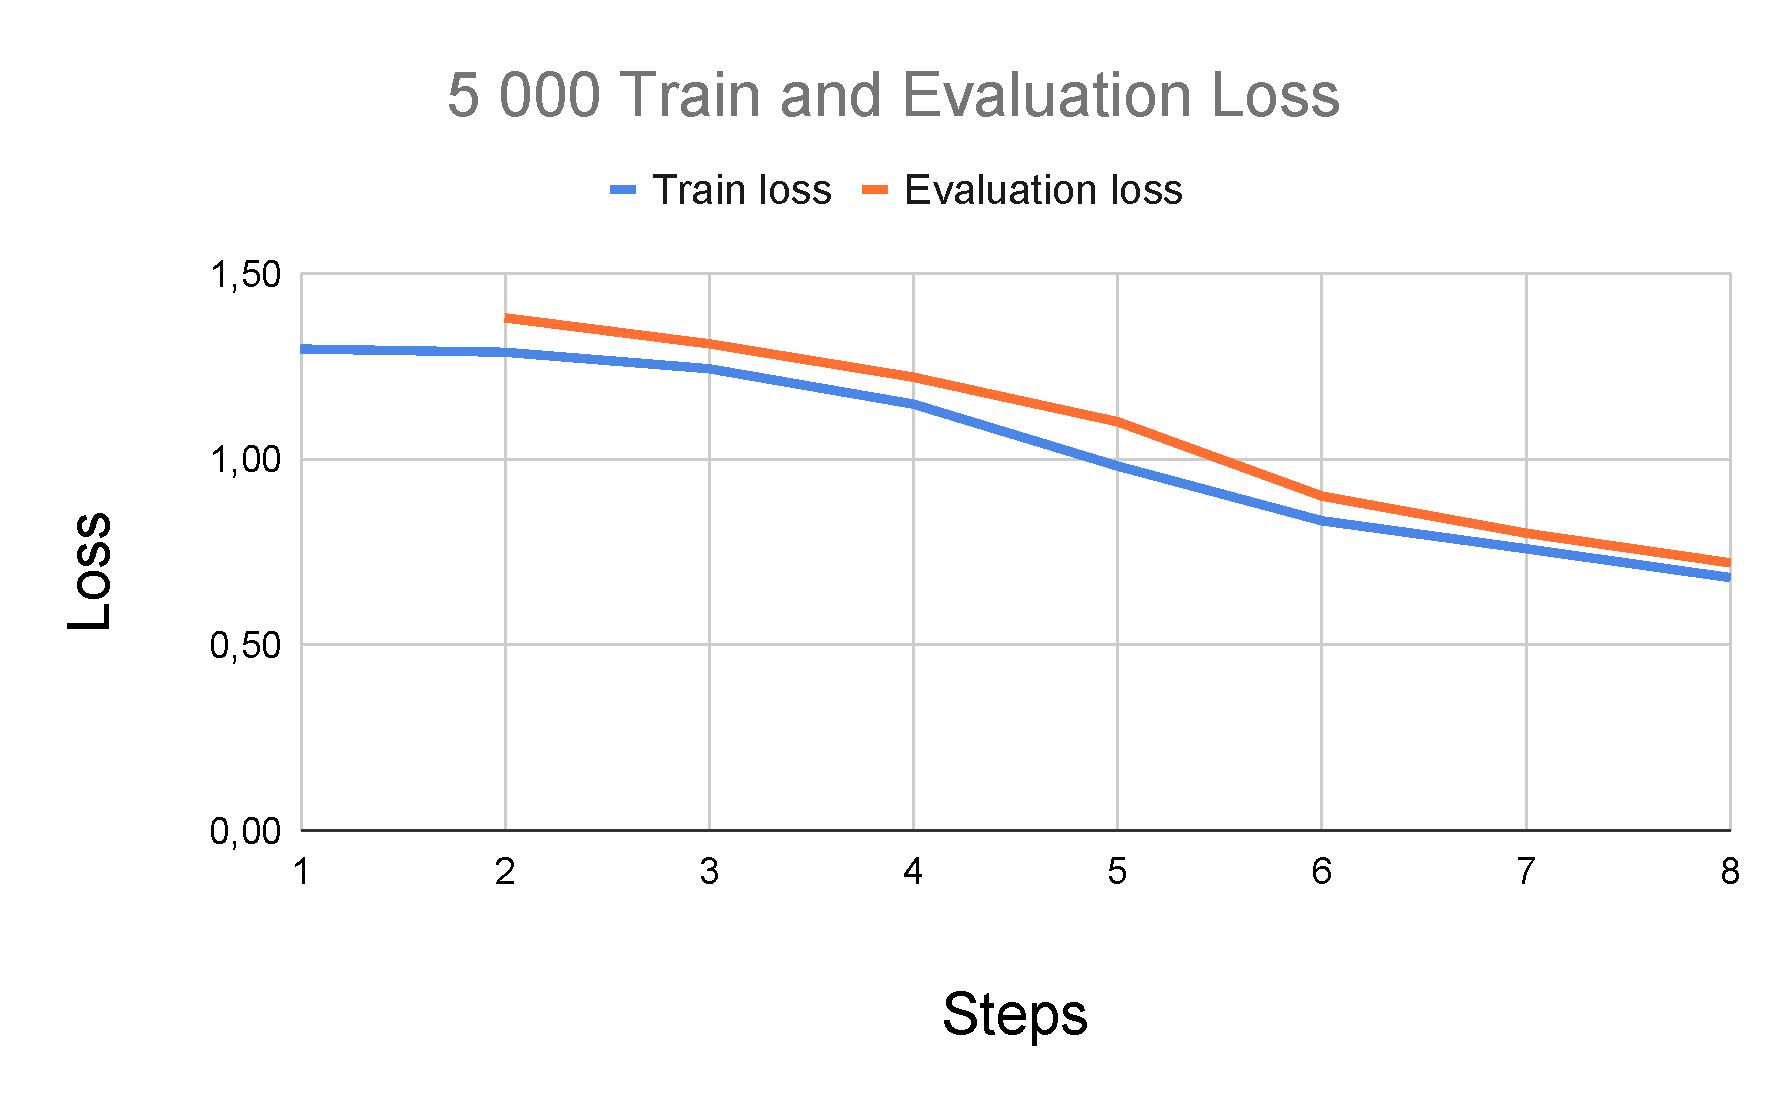
\includegraphics[width=\linewidth]{images/MED-QA-ImageID_5000_samples-Training_loss}
        \caption{Graph over training loss for the initial experiment on 5000 samples.}
        \label{fig:MED-QA-ImageID_5000_samples-Training_loss}
    \end{figure} 


    \subsubsection{Analysis}
    
    It is helpful to analyze the dataset used in training to investigate why the model often answers with "Not relevant".
    When analyzing the correct answers in the dataset, as seen in \autoref{fig:ImageCLEFmed-MEDVQA-GI-2023_answer_label_balance}, it can be seen that the dataset is unbalanced and has a majority of correct answers being "Not relevant". This dataset can be balanced by either over-sample the non-majority classes or under-sample the abundant class, making the model learn that "Not Relevant" is not the best answer in 21,7\% of all questions.
    Going further in the following experiments, the original dataset will be modified. The class "Not relevant" is removed, and the rest of the dataset stays the same. The rationale behind not doing any additional sampling modifications is to reflect the natural occurrences of question-answer pairs in the original dataset. Since this dataset is based on real-world examinations in a hospital, the number of occurrences in the dataset could reflect the real-world occurrence of these findings. In contrast, if this dataset were made synthetically and did not have biases from real-world examinations, there would be more reasonable to modify the number of occurrences of the classes to get a better fit. 
    
    The Alpaca-VQA model will be trained on a larger dataset in the next section. 
    This is to explore how well it can fit the available data and which insights can be gained.


    \begin{figure}[htb]
        \centerline{
        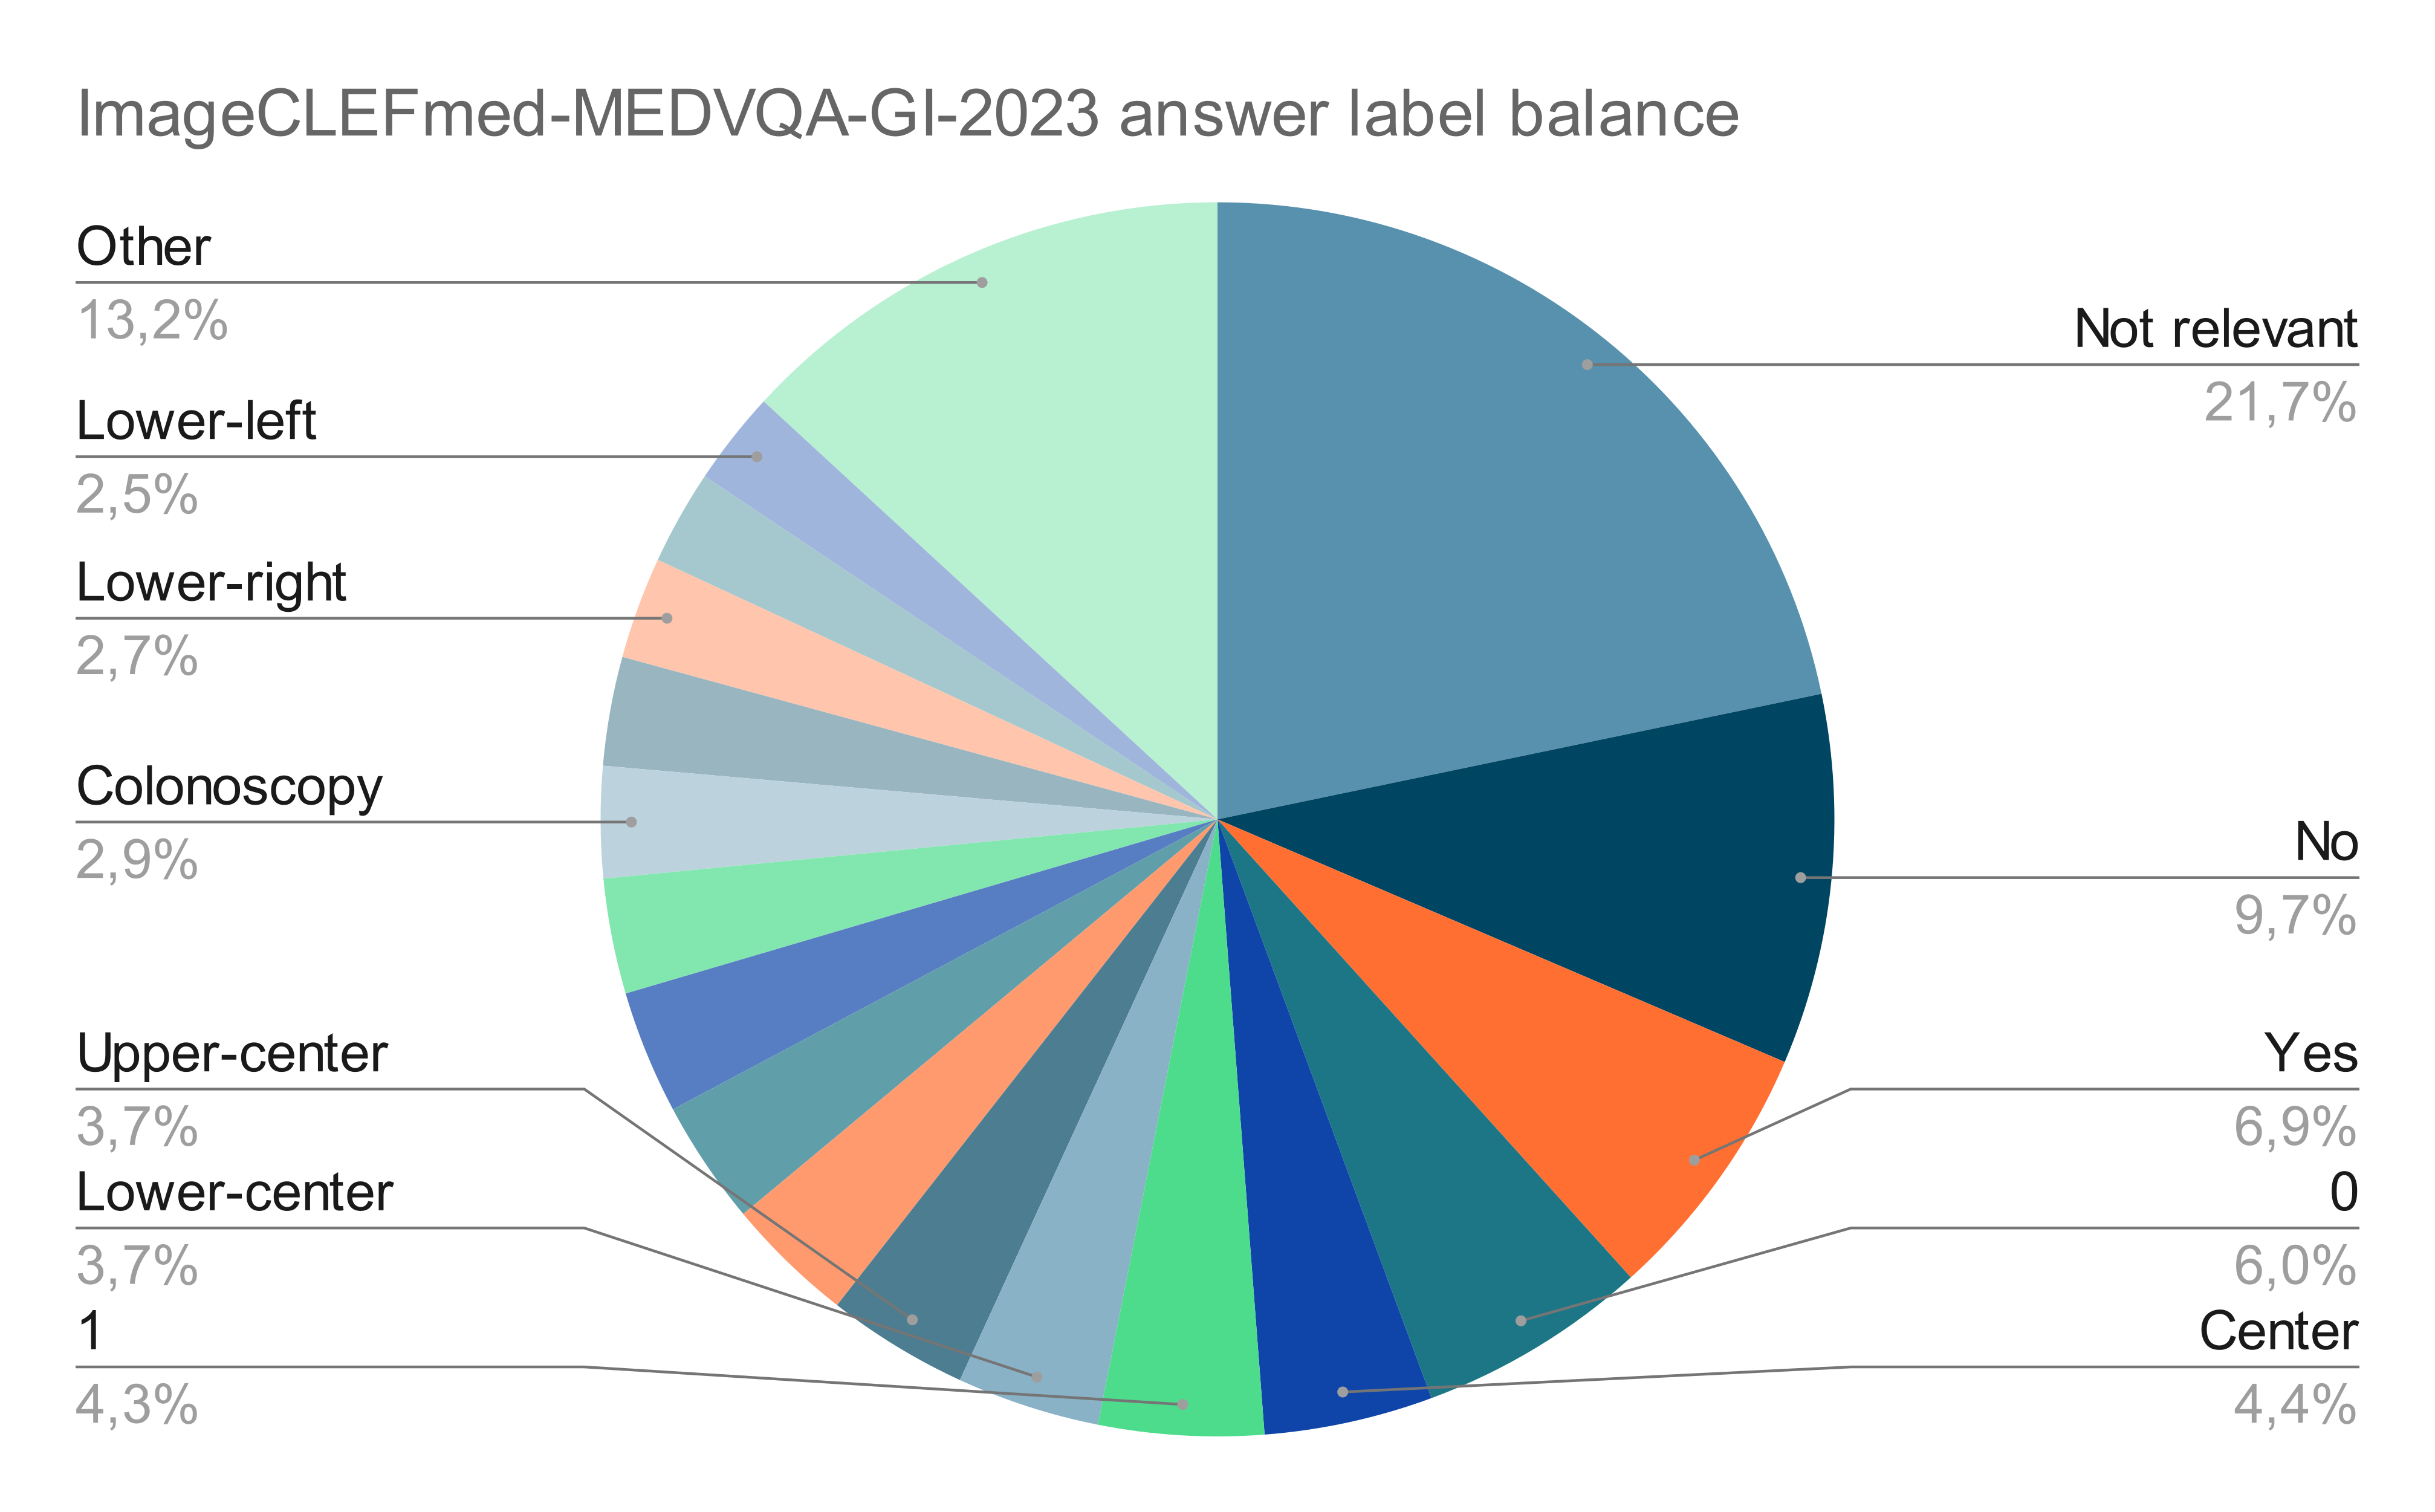
\includegraphics[width=17cm]{images/ImageCLEFmed-MEDVQA-GI-2023_answer_label_balance.png}}
        \caption{Overview of the answer label balance in the ImageCLEFmed-MEDVQA-GI-2023 dataset. 
        %Note that the category "segmentation" is already removed from the dataset due to not being relevant for this task at this stage. 
        The category "Other" is a collection of 46 labels that occur in less than 2,5\% of the samples.}
        \label{fig:ImageCLEFmed-MEDVQA-GI-2023_answer_label_balance}
    \end{figure} 


    \section{Training: 20,000 samples}

    In this experiment, the model is trained on four times as much data as in the investigatory experiment. 
    As noted in the analysis of the previous experiment, the dataset used in this experiment is the same as the original, only with the class "Not relevant" removed.
    Removing this class completely also allows the model to see more relevant data since many of the chosen samples are no longer from the "Not relevant" class. 
    By removing this class, the 20,000 samples will contain more question-answer samples that are relevant to this classification problem. 
    
    The dataset was split as shown in \autoref{fig:dataset_split}, with the original dataset split in two, where the first part was used to train the model, and the second part was used to test and train the proxy model. The reason for leaving half of the dataset unused during the training of the model was to preserve unseen data that could be used to train the proxy model and to test how the model would perform on unseen data. While the model presumably would be able to fit the new task of seeing images given more data, it will still be possible to evaluate if this method is able to interpret image data. How the preserved test data is used to train the proxy model will be discussed later in \autoref{sec4:proxy_lime}.


    \begin{figure}[htb]
        \centerline{
        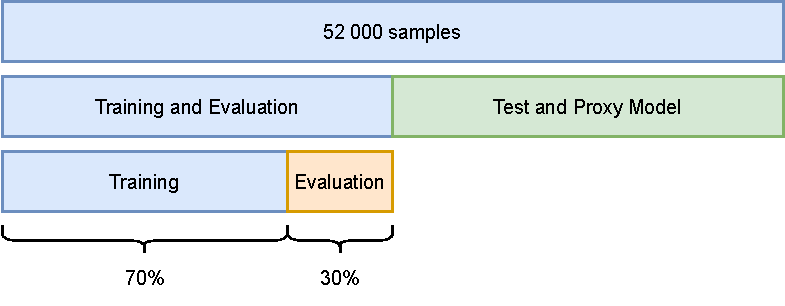
\includegraphics[width=\textwidth]{images/datatset_split.pdf}}
        \caption{Illustration on how the dataset was split into training, evaluation, and testing data.}
        \label{fig:dataset_split}
    \end{figure} 
    
    While training the model on considerably more data would be interesting, the time and computing cost for this experiment would not justify the possible better-trained system, resulting in a more generalized and nuanced model. The experiments carried out with the Alpaca-VQA model are to see how a \gls{llm} would perform on a \gls{vqa} task with image features encoded in the text.
    The final dataset used for training in this experiment contains 20,000 samples, and the class distribution can be seen in \autoref{fig:ImageCLEFmed-MEDVQA-GI-2023_answer_label_balance-modified}.


    The hyperparameters used in this experiment are the same as in the previous experiment and can be seen in \autoref{table:hyperparameters_alpaca}, with a batch size of 256 as previously discussed. While the dataset used in this experiment contains four times more samples than in the previous experiment, the image feature extraction is still the extracted top 100 features from the VGG16 model. 
    Due to the similarities in the data samples, the hyperparameters are kept the same to see how the Alpaca-VQA model responds to a larger dataset.
    
    
    \begin{figure}[htb]
        \centerline{
        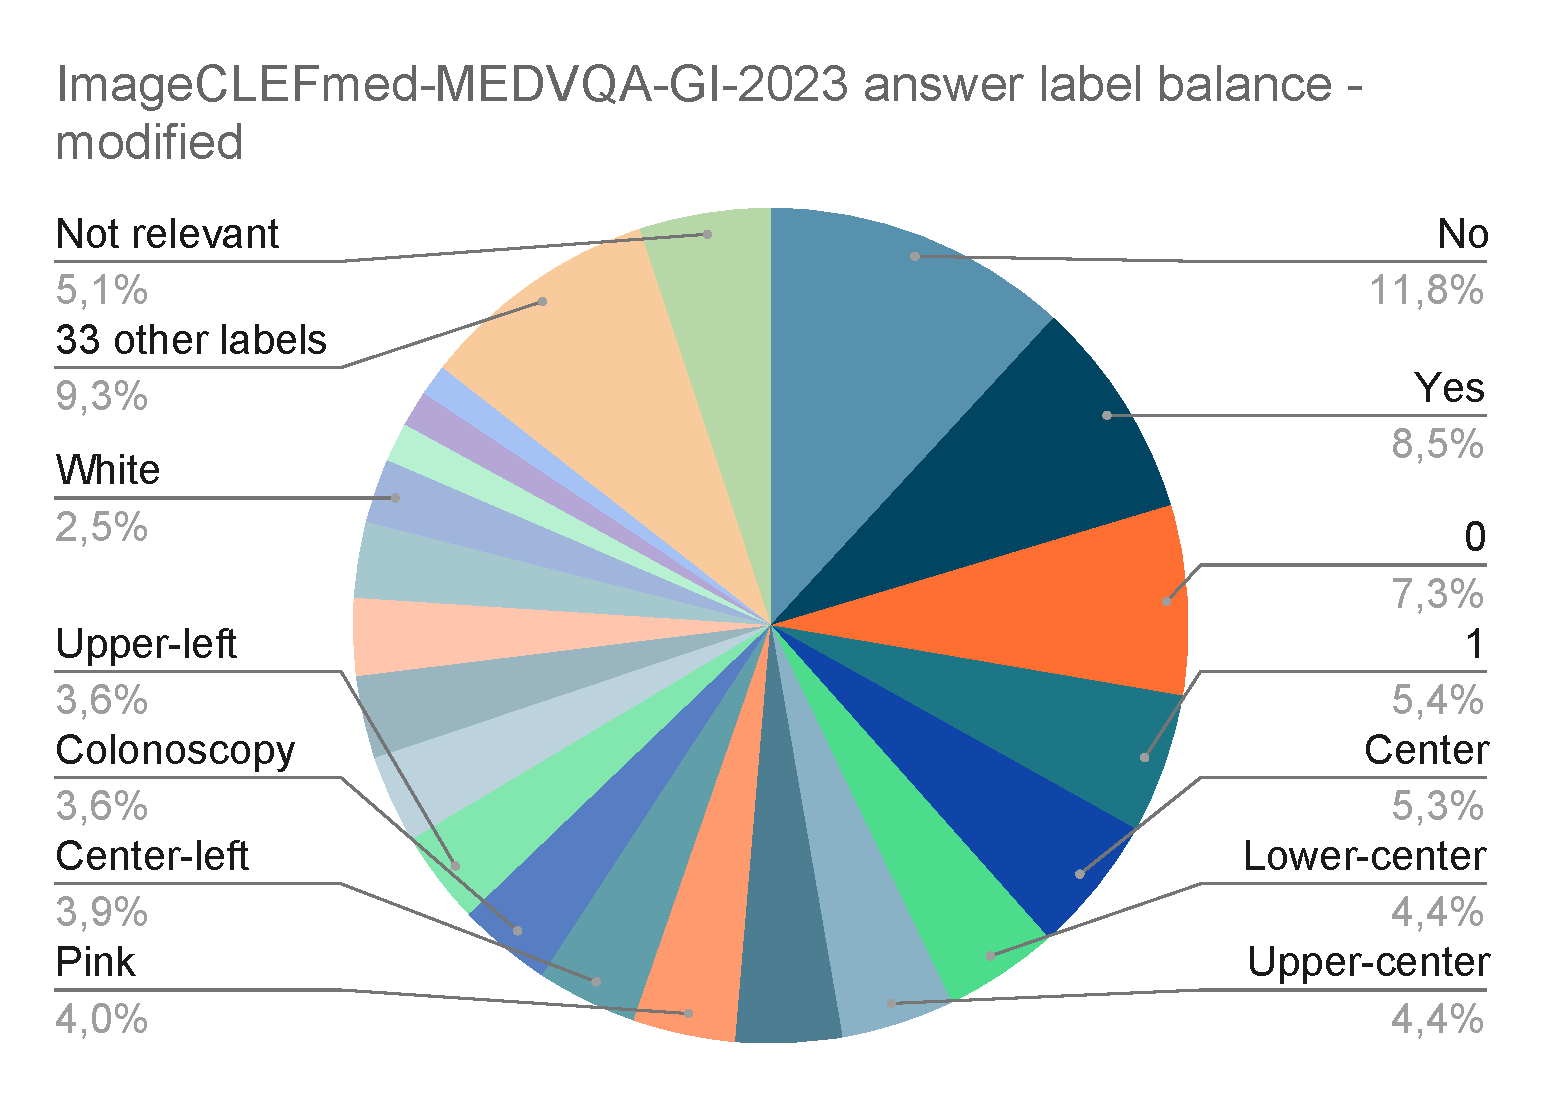
\includegraphics[width=1.08\textwidth]{images/ImageCLEFmed-MEDVQA-GI-2023-answer-label-balance-modified.pdf}}
        \caption{Overview of the answer label distribution in the ImageCLEFmed-MEDVQA-GI-2023 dataset, modified with the class "Not relevant" removed. The category "Other" is a collection of 33 smaller labels in the training data and is only used in this visualization, and is not an actual class.}
        \label{fig:ImageCLEFmed-MEDVQA-GI-2023_answer_label_balance-modified}
    \end{figure} 

    Because of the larger dataset, more evaluation steps were used to help the model correct during training. In the investigatory experiment, 8 steps were used during the runtime. In this training session, with four times as much training data, the number of steps was chosen to be every 10\textsuperscript{th} training step, resulting in 46 evaluation steps in total. 

    \begin{figure}[htb]
        \centerline{
        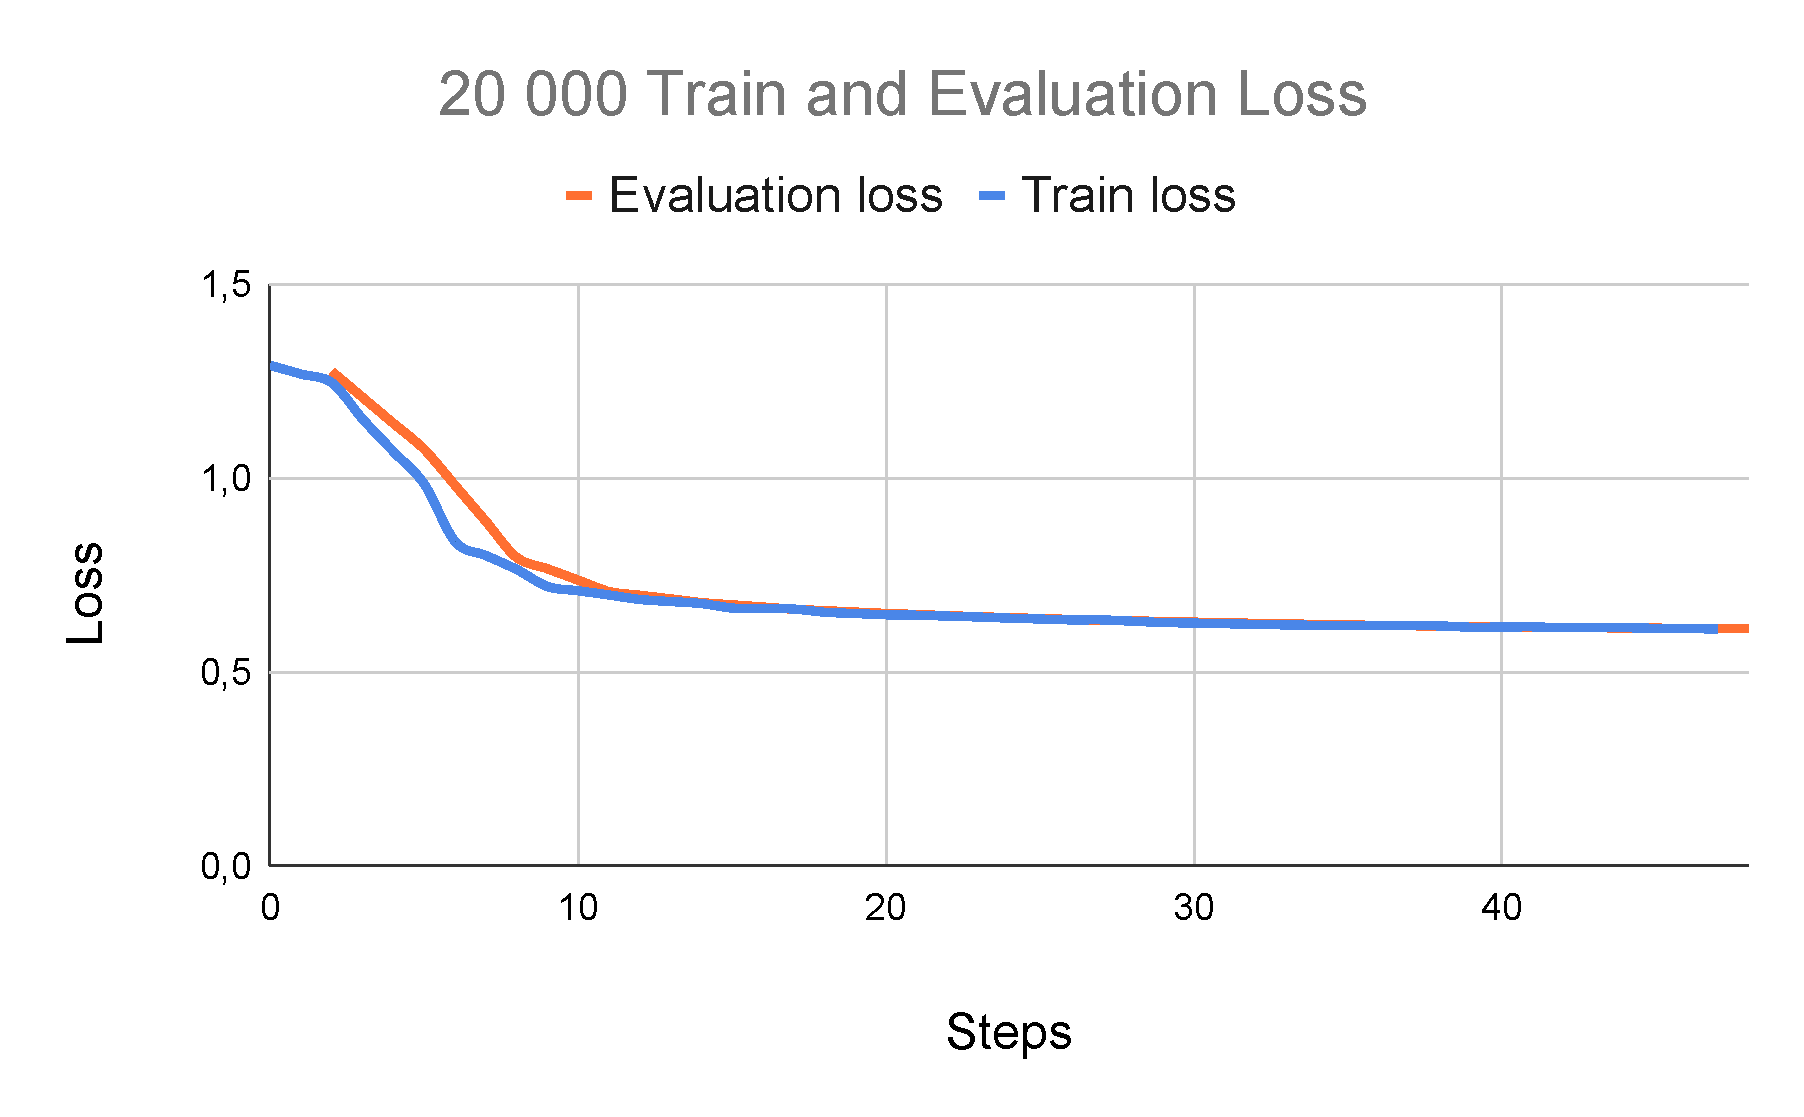
\includegraphics[width=1.07\textwidth]{images/20k_train_evaluation_loss}}
        \caption{Graph over training loss for 20,000 samples.}
        \label{fig:20k_train_eval_loss}
    \end{figure} 
    
    The Alpaca-VQA model on 20,000 samples was trained on an Nvidia A100 with 40 GB \gls{vram}. It took fifteen and a half hours to run, including image encoding, fine-tuning, and evaluating the model. 



    \section{Results}
    \label{sec4:results}
    This section evaluates the results for the Alpaca-VQA model trained on 20,000 samples, where 70\% was used as training data and 30\% as evaluation. The training results will be discussed alongside the classification report, transition scores, proxy model, and a blinded model.
    
    First, the training and evaluation loss graph during this training session can be seen in \autoref{fig:20k_train_eval_loss}. In this graph, it can be seen that the model converges relatively fast and stabilizes during the training run. This can indicate that the model was able to fit the available training data and fine-tune its \gls{lora} update matrices to the training data. Regarding the number of evaluation steps, it can be seen that the evaluation loss is approximately the same as the training loss at step 10. At this step, it can also be seen that the loss for both training and evaluation flattens out. This can indicate that the model has fitted its parameters to the available data and did not have more quality data to learn from. 


    \subsection{Classification Report}
        In order to test how the model was able to fit the training data, a test set was used. The test set was from the same dataset as the training data but naturally did not overlap with the training and evaluation data. 

        As the test result should be used later in order to fit a proxy model, the test set was chosen to be 20,000 samples. These samples should not be confused with the ones used for training and evaluation, as the dataset was split, as previously shown in \autoref{fig:dataset_split}.

        The classification report is shown in \autoref{tab:classification_report_20}. The columns are class labels, the precision, recall, and $F_1$ scores for each class, and the number of occurrences of each class in the test set in the column "Support". At the bottom of the table, the accuracy and average score are calculated. As noted in this table, the Alpaca-VQA scores an accuracy of 29\% on the test set. The number of occurrences in each class shows that this test set is also unbalanced and has approximately the same distribution as the training set.
        
        A simplified table can be found given that \autoref{tab:classification_report_20} is a large table that can be hard to interpret.
        As the $F_1$ score is a harmonic mean of the precision and recall, it can be used to indicate how well the model performs in each class. By removing the classes where the $F_1$ score is 0 from \autoref{tab:classification_report_20}, the result is a simplified representation that can be seen in \autoref{tab:classification_report_20_simpl}.
        From this table, it can be more clearly seen that the classes the trained model performs well on have a high presence in the training set, as previously shown in \autoref{fig:ImageCLEFmed-MEDVQA-GI-2023_answer_label_balance-modified}. Logically, the model performs better on data it has seen and not as well on data it has not been exposed to. From the difference between the full \autoref{tab:classification_report_20} and the simplified \autoref{tab:classification_report_20_simpl}, it can also be seen that despite having relatively high occurrence in both training and testing sets, the Alpaca-VQA model falsely categorizes classes with localization and color labels.
        One possible explanation for this is that the image encoder, the VGG16 model, does not have localization abilities, as it is not designed to output \gls{roi} or multiple objects with bounding boxes. As it is not fine-tuned on the images in this dataset but rather pretrained on ImageNet, the predicted classes may not correlate with colors.
        \begin{center}
\begin{longtable}{|c|c|c|c|c|}
\caption{Classification Report on Test Set - Model trained on 20'000 question-answer pairs.} \label{tab:classification_report_20} \\

\hline \multicolumn{1}{|c|}{\textbf{Class}} & \multicolumn{1}{c|}{\textbf{Precision}} & \multicolumn{1}{c|}{\textbf{Recall}} & \multicolumn{1}{c|}{\textbf{F1-score}} & \multicolumn{1}{c|}{\textbf{Support}}\\ \hline 
\endfirsthead

\multicolumn{3}{c}%
{{\bfseries \tablename\ \thetable{} -- continued from previous page}} \\
\hline \multicolumn{1}{|c|}{\textbf{Class}} & \multicolumn{1}{c|}{\textbf{Precision}} & \multicolumn{1}{c|}{\textbf{Recall}} & \multicolumn{1}{c|}{\textbf{F1-score}} & \multicolumn{1}{c|}{\textbf{Support}}\\ \hline 
\endhead

\hline \multicolumn{5}{|r|}{{Continued on next page}} \\ \hline
\endfoot

\hline \hline
\endlastfoot




0 & 0.54 & 0.92 & 0.68 & 1551 \\
1 & 0.52 & 0.16 & 0.25 & 1132 \\
11-20mm & 0.00 & 0.00 & 0.00 & 97 \\
2 & 0.00 & 0.00 & 0.00 & 306 \\
3 & 0.00 & 0.00 & 0.00 & 13 \\
4 & 0.00 & 0.00 & 0.00 & 2 \\
5 & 0.00 & 0.00 & 0.00 & 2 \\
5-10mm & 0.00 & 0.00 & 0.00 & 100 \\
< 5mm & 0.00 & 0.00 & 0.00 & 55 \\
>20mm & 0.00 & 0.00 & 0.00 & 71 \\
Biopsy forceps & 0.00 & 0.00 & 0.00 & 43 \\
Black & 0.00 & 0.00 & 0.00 & 9 \\
Blue & 0.00 & 0.00 & 0.00 & 4 \\
Brown & 0.00 & 0.00 & 0.00 & 10 \\
Cecum & 0.00 & 0.00 & 0.00 & 33 \\
Center & 0.00 & 0.00 & 0.00 & 1121 \\
Center-left & 0.10 & 0.14 & 0.12 & 831 \\
Center-right & 0.11 & 0.43 & 0.17 & 861 \\
Colonoscopy & 0.98 & 0.05 & 0.10 & 761 \\
Gastroscopy & 0.00 & 0.00 & 0.00 & 242 \\
Green & 0.00 & 0.00 & 0.00 & 3 \\
Grey & 0.00 & 0.00 & 0.00 & 16 \\
Ileum & 0.00 & 0.00 & 0.00 & 2 \\
Injection needle & 0.00 & 0.00 & 0.00 & 1 \\
Lower-center & 0.00 & 0.00 & 0.00 & 938 \\
Lower-left & 0.00 & 0.00 & 0.00 & 616 \\
Lower-right & 0.11 & 0.06 & 0.08 & 769 \\
Metal clip & 0.00 & 0.00 & 0.00 & 11 \\
No & 0.66 & 0.46 & 0.54 & 2505 \\
Oesophagitis & 1.00 & 0.00 & 0.01 & 240 \\
Orange & 0.00 & 0.00 & 0.00 & 16 \\
Pale Pink & 0.00 & 0.00 & 0.00 & 1 \\
Paris iia & 0.00 & 0.00 & 0.00 & 95 \\
Paris ip & 0.00 & 0.00 & 0.00 & 101 \\
Paris is & 0.00 & 0.00 & 0.00 & 125 \\
Pink & 0.38 & 0.04 & 0.07 & 819 \\
Polyp & 0.25 & 0.96 & 0.39 & 311 \\
Polyp snare & 0.00 & 0.00 & 0.00 & 30 \\
Purple & 0.00 & 0.00 & 0.00 & 1 \\
Pylorus & 0.00 & 0.00 & 0.00 & 1 \\
Red & 0.29 & 0.27 & 0.28 & 629 \\
Tube & 0.00 & 0.00 & 0.00 & 218 \\
Ulcerative colitis & 0.00 & 0.00 & 0.00 & 250 \\
Upper-center & 0.00 & 0.00 & 0.00 & 944 \\
Upper-left & 0.00 & 0.00 & 0.00 & 764 \\
Upper-right & 0.11 & 0.38 & 0.16 & 729 \\
White & 0.00 & 0.00 & 0.00 & 520 \\
Yellow & 0.02 & 0.06 & 0.03 & 79 \\
Yes & 0.59 & 0.98 & 0.74 & 1778 \\
Z-line & 0.00 & 0.00 & 0.00 & 220 \\
Brown & 0.00 & 0.00 & 0.00 & 4 \\
Grey & 0.00 & 0.00 & 0.00 & 7 \\
Purple & 0.00 & 0.00 & 0.00 & 3 \\
\hline
Accuracy &  &  & 0.29 & 20000 \\
Macro average & 0.09 & 0.08 & 0.06 & 20000 \\
Weighted average & 0.30 & 0.29 & 0.24 & 20000 \\

\end{longtable}
\end{center}
        \begin{center}
\begin{longtable}{|c|c|c|c|c|}
\caption{Simplified Classification Report on Test Set, only non-zero $F_1$ scores - Model trained on 20,000 question-answer pairs.} \label{tab:classification_report_20_simpl} \\

\hline \multicolumn{1}{|c|}{\textbf{Class}} & \multicolumn{1}{c|}{\textbf{Precision}} & \multicolumn{1}{c|}{\textbf{Recall}} & \multicolumn{1}{c|}{\textbf{F1-score}} & \multicolumn{1}{c|}{\textbf{Support}}\\ \hline 
\endfirsthead

\multicolumn{3}{c}%
{{\bfseries \tablename\ \thetable{} -- continued from previous page}} \\
\hline \multicolumn{1}{|c|}{\textbf{Class}} & \multicolumn{1}{c|}{\textbf{Precision}} & \multicolumn{1}{c|}{\textbf{Recall}} & \multicolumn{1}{c|}{\textbf{F1-score}} & \multicolumn{1}{c|}{\textbf{Support}}\\ \hline 
\endhead

\hline \multicolumn{5}{|r|}{{Continued on next page}} \\ \hline
\endfoot

\hline \hline
\endlastfoot

0 & 0.54 & 0.92 & 0.68 & 1551 \\
1 & 0.52 & 0.16 & 0.25 & 1132 \\
Center-left & 0.10 & 0.14 & 0.12 & 831 \\
Center-right & 0.11 & 0.43 & 0.17 & 861 \\
Colonoscopy & 0.98 & 0.05 & 0.10 & 761 \\
No & 0.66 & 0.46 & 0.54 & 2505 \\
Oesophagitis & 1.00 & 0.00 & 0.01 & 240 \\
Pink & 0.38 & 0.04 & 0.07 & 819 \\
Polyp & 0.25 & 0.96 & 0.39 & 311 \\
Red & 0.29 & 0.27 & 0.28 & 629 \\
Upper-right & 0.11 & 0.38 & 0.16 & 729 \\
Yellow & 0.02 & 0.06 & 0.03 & 79 \\
Yes & 0.59 & 0.98 & 0.74 & 1778 \\

\end{longtable}
\end{center}

        The classification reports are just a score on the top-level prediction of the model and do not give insight into why or how the model classifies labels. The next two subsections present different approaches to gaining insight into how the model predicts its answers. Having ways to present how the model works can aid in determining how much a user can trust the answers given by a system. 
    
    
    \subsection{Visualizing Transition Scores}
    \label{sec4:vis_transtion_scores}

    \begin{comment}
        Furthermore, analyzing the transition scores can help identify cases of hallucination or incorrect reasoning in the model's responses. If the model assigns high attention weights to irrelevant or incorrect parts of the input, it may indicate that it generates answers based on incorrect or unrelated information.
    \end{comment}
   
    This subsection explores the transition scores given by the Alpaca-VQA model when it generates its answers. These scores can provide valuable insights into how the model processes and generates its responses. This insight can help understand which words or tokens in the input are most influential when generating an answer. 
    Transition scores represent the attention or importance given to the different parts of the input sequence when generating new tokens in the output. Visualizing the transition scores can also reveal patterns and biases in the model's attention mechanism, like if the attention biases specific tokens.
    
    As the Alpaca-VQA model uses the transformer architecture from HuggingFace, implementing the transition scores is as simple as \autoref{code:transition_scores}

\begin{lstlisting}[language=Python, caption=Example of how to generate transition scores, label={code:transition_scores}]
# Generate output tokens
generation_output = model.generate(
    input_ids=input_ids,
    generation_config=generation_config,
    return_dict_in_generate=True,
    output_scores=True,
    max_new_tokens=256,
    temperature=0.1,
    top_p=0.75,
    top_k=40,
    num_beams=4,
)

# Compute transition scores
transition_scores = model.compute_transition_scores(
    generation_output.sequences, 
    generation_output.scores, 
    normalize_logits=True
)
\end{lstlisting}

    \begin{table}[htb]
        \small
        \centering
        \begin{tabularx}{\textwidth}{ @{} m{4cm}  M{3cm}  Y  Y @{} }
            \multicolumn{4}{c}{\textbf{Transition Scores}}\\ 
            \toprule 
            Question & Ground Truth & Predicted Token & Transition Score \\
            \midrule
            
            Are there any anatomical landmarks in the image? & No & No & 21.20\%\\
        \noalign{\vskip 2mm} 
        \cline{1-4}
        \noalign{\vskip 2mm}    
        
          \multirow{3}{=}{Where in the image is the instrument?} & \multirow{3}{*}{Upper-left} & Lower & 50.49\% \\
             &  & - & 99.76\%\\ 
             &  & left & 40.16\% \\
        \noalign{\vskip 2mm} 
        \cline{1-4}
        \noalign{\vskip 2mm}    
          How many polyps are in the image? & 0 & 0 & 90.38\%\\
        \noalign{\vskip 2mm} 
        \cline{1-4}
        \noalign{\vskip 2mm}    
          \multirow{4}{=}{What type of procedure is the image taken from?} & 
          \multirow{4}{*}{Laparoscopy} & Comput & 53.12\% \\
             &  & ed & 47.85\%\\ 
            &  & tom & 97.61\%\\ 
             &  & ography & 99.41\% \\
        
        \noalign{\vskip 2mm} 
        \cline{1-4}
        \noalign{\vskip 2mm}    
        
          \multirow{4}{=}{What type of polyp is present?} & 
          \multirow{4}{*}{Paris is} & Par & 19.25\% \\
             &  & ap & 41.16\%\\ 
            &  & lex & 71.34\%\\ 
             &  & is & 46.92\% \\
        \noalign{\vskip 2mm} 
        \cline{1-4}
        \noalign{\vskip 2mm}    
          \multirow{4}{=}{What type of procedure is the image taken from?} & 
          \multirow{4}{*}{Colonoscopy} & Col & 19.29\% \\
            &  & on & 99.80\%\\ 
            &  & os & 100.00\%\\ 
            &  & copy & 99.90\% \\
            \bottomrule
        \end{tabularx}
        \caption{Examples of transition scores computed by Alpaca-VQA. All questions were asked in relation to an image input.}
        \label{table:transition_score}
    \end{table}


    In \autoref{table:transition_score}, examples of transition scores computed by Alpaca-VQA on various questions are displayed.
    These scores should be seen in conjunction with the distribution of classes in the training set, which was previously discussed and can be seen in \autoref{fig:ImageCLEFmed-MEDVQA-GI-2023_answer_label_balance-modified}. 
    As the model uses the connections made during training when predicting answers, the transition scores with high probability are usually from one of the majority classes in the training set. Examples of these, as shown in \autoref{table:transition_score} are "Lower" and "0". 
    It can also be seen how the Alpaca-VQA model splits up words into tokens, like how \textit{"Computed Tomography"} gets split into tokens that can be used in other words. For example, the token \textit{"comput"} be used in words like \textit{"computer"}, \textit{"computed"}, \textit{"computing"}, and so on. By splitting the words into non-redundant tokens, the tokenizer keeps the dictionary of tokens efficient. 

    An interesting finding is that the predicted answers are not always from the fine-tuning dataset. In \autoref{table:transition_score}, the predicted answers \textit{"Computed Tomography"} and \textit{"Paraplexis"} does not occur in the dataset Alpaca-VQA is fine-tuned on, namely ImageCLEFmed-MEDVQA-GI-2023. 
    It can also be seen in the case of \textit{"Paraplexis"} that the model correctly identifies the first token, \textbf{par}, although with a low score. Then the model follows up with the tokens it thinks finish the word by predicting \textit{ed} with a 47,85\% score. Most likely, \textit{"Paraplexis"} was predicted by having a higher average score in the four beams than the correct answer. As the training data has multiple instances of the Paris classification system, potentially diluting the importance of the polyp class following the prefix "Paris".
    
    The base model of Alpaca-VQA, the Stanford Alpaca, is a fine-tuned instruction-following model based on the \gls{llama} 7 billion parameters model. Upon investigation, \textit{"Computed Tomography"} and \textit{"Paraplexis"} are not part of this instruction-following fine-tuning dataset either. Therefore the knowledge of these medical subjects originates from the original \gls{llama} model. As noted in \autoref{table:llama_pre_train_data} on Page \pageref{table:llama_pre_train_data}, the dataset used for pre-training the \gls{llama} model is disclosed and based on publicly available data, but not made public as the time of writing. Therefore it can not be known exactly where this information stems from, other than from the dataset used for pre-training the \gls{llama} 7B model.


     \begin{figure}[htb]
        \centerline{
        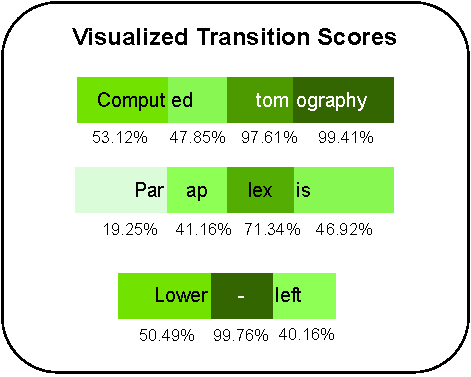
\includegraphics[width=0.65\textwidth]{images/visualized_transition_scores.pdf}}
        \caption{The Alpaca-VQA transition scores visualized.}
        \label{fig:visualized_transition_scores}
    \end{figure} 


    When using the transition scores calculated, the scores can be seen as a decimal value between zero and one. This value can be used as a weight when applying color to each individual token. Some of the predicted answers from \autoref{table:transition_score} are visualized using this method in \autoref{fig:visualized_transition_scores}.

    As transition scores can be useful to get insight into how confident the model is when predicting a token, visualizing the scores can make them more intuitive for a user. Instead of only presenting the transition scores as percentages, colors are more often understood by non-technical users. By making more of the model presentable in an intuitive way, more users can gain insight into how it works and where it can be improved. 
    The next subsection will explain another way to make models more transparent and presentable to humans. The experiment uses a proxy model explained by \gls{lime}. 
    
    
    
    \subsection{Proxy model and LIME}
    \label{sec4:proxy_lime}
    This subsection will describe how the proxy model and \gls{lime} method were adapted to give insight into how the Alpaca-VQA model works.
    
    \subsubsection{Proxy model}
    The proxy model used to interpret the Alpaca-VQA model was trained on the predicted outputs of the \gls{llm}. These answers were generated using half of the available dataset, as shown in \autoref{fig:dataset_split}. The rationale behind this was to see how well the Alpaca-VQA model performed on unseen data that could be used to fit the proxy model so that it mimics the underlying model. 
    The available test set of 20,000 samples with predicted answers by the Alpaca-VQA model was used as a training and testing set for the proxy model. The dataset was split into roughly 70\% training data and 30\% evaluation data. Because a random split was used, the precise numbers used were 14,351 for the training set and 5649 for the test set.
    The proxy model is a \gls{sdg} classifier implemented by SciKit Learn \cite{SklearnLinearModel}.
    The hyperparameters used when training the proxy model are shown in \autoref{table:proxy_params}. Mostly the parameters used are the default for this implementation of the model, with the most notable difference being that the loss function is a modified Huber instead of the default \textit{hinge}, giving a linear \gls{svm}. 
    The modified Huber is a smooth loss function that brings tolerance to
    outliers as well as probability estimates, and was chosen because it gave the best results among the available loss functions.
    

    \begin{table}[htb]
    \centering
    \begin{tabular}{ r c } 
        \multicolumn{2}{c}{\textbf{\gls{sdg} Classifier Hyperparameters}}\\ 
        \toprule
           Hyperparameter & Value \\
        \midrule
            Loss: & Modified Huber\\
            Penalty: & $L_2$\\
            Alpha: & $1e^{-3}$\\
            Random state: & 42\\
            Max iterations: & 1000\\
            Class weight: & Balanced\\[0.5ex]
        \bottomrule
    \end{tabular}
    \caption{Overview of the parameters used when training the proxy model.}
    \label{table:proxy_params}
    \end{table}
    

    A classification report was made when the \gls{sdg} classifier, used as a proxy model, was fitted. This report can be seen in \autoref{tab:classification_report_proxy}, and it can be seen that the model fits the Alpaca-VQA model with a satisfactory accuracy of 84\%. This score indicates that the proxy model will answer the same as the Alpaca-VQA model approximately 86\% of the time, given the same questions and images.

    \begin{center}
\begin{longtable}{|c|c|c|c|c|}
\caption[Classification Report: Proxy Model.]{Proxy Model Classification Report} \label{tab:classification_report_proxy} \\

\hline \multicolumn{1}{|c|}{\textbf{Class}} & \multicolumn{1}{c|}{\textbf{Precision}} & \multicolumn{1}{c|}{\textbf{Recall}} & \multicolumn{1}{c|}{\textbf{F1-score}} & \multicolumn{1}{c|}{\textbf{Support}}\\ \hline 
\endfirsthead

\multicolumn{3}{c}%
{{\bfseries \tablename\ \thetable{} -- continued from previous page}} \\
\hline \multicolumn{1}{|c|}{\textbf{Class}} & \multicolumn{1}{c|}{\textbf{Precision}} & \multicolumn{1}{c|}{\textbf{Recall}} & \multicolumn{1}{c|}{\textbf{F1-score}} & \multicolumn{1}{c|}{\textbf{Support}}\\ \hline 
\endhead

\hline \multicolumn{5}{|r|}{{Continued on next page}} \\ \hline
\endfoot

\hline \hline
\endlastfoot

0 &   0.87 &  0.98 &  0.92 &   783 \\
1 &   0.00 &  0.00 &  0.00 &   111 \\
2-3mm &   0.00 &  0.00 &  0.00 &     0 \\
3-5mm &   0.99 &  1.00 &  0.99 &    99 \\
Center-left &   0.77 &  0.85 &  0.81 &   336 \\
Center-right &   0.94 &  0.74 &  0.83 &  1,059 \\
Colonoscopy &   0.00 &  0.00 &  0.00 &     9 \\
Endoscopy &   0.67 &  0.94 &  0.78 &   185 \\
Laparoscopy &   0.14 &  0.04 &  0.06 &    60 \\
Lower-right &   0.44 &  0.94 &  0.60 &    98 \\
No &   0.98 &  0.93 &  0.95 &   532 \\
Oesophagitis &   0.00 &  0.00 &  0.00 &     0 \\
Pink &   0.29 &  0.64 &  0.40 &    28 \\
Polyp &   0.97 &  0.77 &  0.86 &   343 \\
Polypus &   0.23 &  0.95 &  0.38 &    22 \\
Red &   0.90 &  0.97 &  0.93 &   178 \\
Upper-right &   0.86 &  0.84 &  0.85 &   784 \\
Yellow &   0.62 &  0.73 &  0.67 &    74 \\
Yes &   0.97 &  0.96 &  0.96 &   893 \\
Biopsy &   0.00 &  0.00 &  0.00 &     1 \\
Endoscopy &   0.45 &  0.30 &  0.36 &    44 \\
Yellow &   0.17 &  1.00 &  0.29 &    10 \\
\hline
Accuracy &  &   &   0.84 &  5,649 \\
Macro average &   0.49 &  0.59 &  0.51 &  5,649 \\
Weighted average &   0.86 &  0.84 &  0.84 &  5,649 \\
 

\end{longtable}
\end{center}


    \subsubsection{Explaining the proxy model with LIME}
    
    In order to interpret this proxy model, the \gls{xai} method \gls{lime} was fitted. Specifically, the TextExplainer module \cite{LimePackageLime} was used to adapt to the proxy model, and the default parameters for TextExplainer were used. The TextExplainer uses as default an exponential kernel that uses a cosine distance metric and only uses words present in the text as explanations. This restriction helps speed up the explanation process, as only the relevant words are used, and not the whole vocabulary of the \gls{llm}. 

    In order to explain the proxy model, the \gls{lime} method first generates a neighborhood of the data by hiding features randomly from the explaining instance. Then the explaining instance uses this neighborhood to learn locally weighted linear models that explain each class. By learning these linear models, the \gls{lime} instance can interpret which word has a high impact on the predicted outcome. 
    
    
    As the stacked model design of this explanation pipeline can obscure the underlying Alpaca-VQA model, there are still some insights to be had. The \gls{lime} model is designed to give locally accurate interpretations of which parameters the underlying model uses. Therefore, the \gls{lime} model should be transparent to the proxy model. However, the proxy model has no transparency of which features it bases its decisions on. 
    The similarities between the Alpaca-VQA model and the proxy model are that they both are trained on data from the same dataset and sample distribution, with the proxy model ignoring ground truth and using the predicted answer from Alpaca-VQA as its correct answer. 
    Therefore, the proxy model does not give a locally accurate representation of the inner workings of the underlying model and may weigh the inputs differently than the Alpaca-VQA model. 
    Yet, as the proxy model is trained to mimic the underlying model and fits with an accuracy of 86\%, there is still a possibility that the proxy model can give insight into how the \gls{llm} work and possibly exploit biases in the dataset.

    The outcome of the proxy model being explained by \gls{lime} for one instance can be seen in \autoref{fig:lime_crop}. Here it can be seen that the \gls{lime} instance predicts that the input question is most relevant in answering the question. The ground truth answer can be seen in the top left corner of this figure, together with the predicted answer by Alpaca-VQA and the proxy model. In this figure \gls{lime} highlights words that have a high impact on the outcome. The four most probable classes are visualized to the left in the image. The class "Other" is how the \gls{lime} instance classifies the possibility of the predicted class not being in the top four.
    In the \autoref{fig:lime_crop}, it can be seen that the class "Red" is thought to have the highest probability of being correct. In the middle of the figure, the two most probable classes are explained by visualizing the positive and negative impact different words have on the outcome. The figure shows that both "Red" and "Yellow" mostly depend on the same words and do not consider the image features.

    
    \begin{figure}[htb]
        \centerline{
        
\includegraphics[width=1.2\textwidth]{images/LIME_crop.pdf}}
        \caption{The proxy model explained by LIME.}
        \label{fig:lime_crop}
    \end{figure} 

    In this experiment with the proxy model explained by \gls{lime}, there is a likelihood that the model only considers the question and ignores the image features when predicting an answer. Since this is an indicator that the model detected some bias in the language used in the questions, the next experiment removes the image from the input entirely. Testing the Alpaca-VQA model trained on question-answer pairs, including image features, and removing the image features during testing, can provide insight into whether the proxy model exploited the same biases as the underlying model.
    
    


    \subsection{Language-only Alpaca-VQA model}
    \label{sec4_language_only_model}
        
        As noted by the authors of the \gls{vqa} 2.0 dataset \cite{goyalMakingVQAMatter2017}, it could be observed that some \gls{vqa} models in their experiments learned biases in the language of the question-answer pairs. This was demonstrated by removing the image altogether from the testing phase and letting the model predict answers only based on the question. Suppose these language-only models perform similarly to the models that also can see images. In that case, it is an indicator that the model has exploited severe language biases and mainly uses these when answering a question. 
        A model that has exploited these language biases will not ground its answers equally on the question and image, resulting in a reduced ability to answer correctly, given that the same question can have multiple images.

        The classification report on 20,000 language-only test samples is listed in \autoref{tab:classification_report_blind}. The model is the same as in the previous reports, but the images are left out when testing.
        As seen in the classification report, the language-only Alpaca-VQA model has an accuracy of 38\% on this test set. Compared to the model that could also see images, the language-only model managed to correctly classify more samples without analyzing images.

        Generally, a model trained on a larger dataset with more parameters is expected to perform better than one trained on a smaller dataset. This performance is because it has more data to learn from, making it able to capture the underlying patterns in the data more precisely. 
        However, there are certain situations where a model trained on a smaller dataset may perform better, and it is usually related to the quality of the dataset. Because the data quality is different, this performance discrepancy can be why the model trained on language-only performs better than on the complete VQA dataset, including images. 
        
        One possible reason is that the smaller dataset, without image features, may have a higher signal-to-noise ratio, meaning the useful data patterns are more precise and distinct. A dataset with a higher signal-to-noise ratio makes it easier for the model to learn and generalize well to new data. In contrast, a larger dataset with more parameters may have more noise or variability, making it harder for the model to distinguish the relevant patterns. 
        More noise may lead to overfitting or poor generalization performance. In this example, from the loss curve, there is a possibility that the Alpaca-VQA model did not generalize well to the available data, as the graph flattens relatively early in the training phase.
        
        Another possible reason is that the samples with fewer features better represent the target distribution or application domain and may capture the key patterns and characteristics relevant to the task. In contrast, a larger dataset may contain more diverse or irrelevant data that can dilute the important signal and affect the performance of the model. One rationale is that the language-only model's higher accuracy can be explained by the fact that the image features are considered noise to the language model and that it can not utilize the information given.

          
        \begin{center}
\begin{longtable}{|c|c|c|c|c|}
\caption[Classification Report: Language-Only Alpaca-VQA.]{Language-Only Alpaca-VQA: Classification Report on 5,000 question-only samples.\\Model trained on 20,000
question-answer pairs, including images. Tested on only questions.} \label{tab:classification_report_blind} \\

\hline \multicolumn{1}{|c|}{\textbf{Class}} & \multicolumn{1}{c|}{\textbf{Precision}} & \multicolumn{1}{c|}{\textbf{Recall}} & \multicolumn{1}{c|}{\textbf{F1-score}} & \multicolumn{1}{c|}{\textbf{Support}}\\ \hline 
\endfirsthead

\multicolumn{3}{c}%
{{\bfseries \tablename\ \thetable{} -- continued from previous page}} \\
\hline \multicolumn{1}{|c|}{\textbf{Class}} & \multicolumn{1}{c|}{\textbf{Precision}} & \multicolumn{1}{c|}{\textbf{Recall}} & \multicolumn{1}{c|}{\textbf{F1-score}} & \multicolumn{1}{c|}{\textbf{Support}}\\ \hline 
\endhead

\hline \multicolumn{5}{|r|}{{Continued on next page}} \\ \hline
\endfoot

\hline \hline
\endlastfoot


0  &   0.70  &  0.91  &  0.79  &  1,551 \\
1  &   0.57  &  0.51  &  0.54  &  1,132 \\
11-20mm  &   0.30  &  1.00  &  0.46  &    97 \\
2  &   0.00  &  0.00  &  0.00  &   306 \\
3  &   0.00  &  0.00  &  0.00  &    13 \\
4  &   0.00  &  0.00  &  0.00   &  2 \\
5  &   0.00  &  0.00  &  0.00   &  2 \\
5-10mm  &   0.00  &  0.00  &  0.00  &   100 \\
< 5mm  &   0.00  &  0.00  &  0.00  &    55 \\
>20mm  &   0.00  &  0.00  &  0.00  &    71 \\
Biopsy forceps  &   0.08  &  1.00  &  0.15  &    43 \\
Black  &   0.00  &  0.00  &  0.00   &  9 \\
Blue  &   0.00  &  0.00  &  0.00   &  4 \\
Brown  &   0.00  &  0.00  &  0.00  &    10 \\
Cecum  &   0.00  &  0.00  &  0.00  &    33 \\
Center  &   0.00  &  0.00  &  0.00  &  1,121 \\
Center-left  &   0.11  &  0.87  &  0.19  &   831 \\
Center-right  &   0.00  &  0.00  &  0.00  &   861 \\
Colonoscopy  &   0.76  &  1.00  &  0.86  &   761 \\
Gastroscopy  &   0.00  &  0.00  &  0.00  &   242 \\
Green  &   0.00  &  0.00  &  0.00   &  3 \\
Grey  &   0.00  &  0.00  &  0.00  &    16 \\
Ileum  &   0.00  &  0.00  &  0.00   &  2 \\
Injection needle  &   0.00  &  0.00  &  0.00   &  1 \\
Lower-center  &   0.00  &  0.00  &  0.00  &   938 \\
Lower-left  &   0.00  &  0.00  &  0.00  &   616 \\
Lower-right  &   0.00  &  0.00  &  0.00  &   778 \\
Metal clip  &   0.00  &  0.00  &  0.00  &    11 \\
No  &   0.73  &  0.38  &  0.50  &  2505 \\
Oesophagitis  &   0.00  &  0.00  &  0.00  &   240 \\
Orange  &   0.00  &  0.00  &  0.00  &    16 \\
Pale Pink  &   0.00  &  0.00  &  0.00   &  1 \\
Paris iia  &   0.30  &  1.00  &  0.46  &    95 \\
Paris ip  &   0.00  &  0.00  &  0.00  &   101 \\
Paris is  &   0.00  &  0.00  &  0.00  &   125 \\
Pink  &   0.39  &  1.00  &  0.56  &   819 \\
Polyp  &   0.00  &  0.00  &  0.00  &   311 \\
Polyp snare  &   0.00  &  0.00  &  0.00  &    30 \\
Purple  &   0.00  &  0.00  &  0.00   &  1 \\
Pylorus  &   0.00  &  0.00  &  0.00   &  1 \\
Red  &   0.00  &  0.00  &  0.00  &   629 \\
Tube  &   0.00  &  0.00  &  0.00  &   218 \\
Ulcerative colitis  &   0.25  &  1.00  &  0.40  &   250 \\
Upper-center  &   0.16  &  0.14  &  0.15  &   944 \\
Upper-left  &   0.00  &  0.00  &  0.00  &   764 \\
Upper-right  &   0.00  &  0.00  &  0.00  &   729 \\
White  &   0.00  &  0.00  &  0.00  &   520 \\
Yellow  &   0.00  &  0.00  &  0.00  &    79 \\
Yes  &   0.71  &  0.80  &  0.75  &  1,778 \\
Z-line  &   0.28  &  1.00  &  0.44  &   220 \\
brown  &   0.00  &  0.00  &  0.00   &  4 \\
grey  &   0.00  &  0.00  &  0.00   &  7 \\
purple  &   0.00  &  0.00  &  0.00   &  3 \\
\hline
Accuracy &  &  & 0.38 &  20,000 \\
Macro average &  0.10 &   0.19 &  0.11 &   20,000 \\
Weighted average  &  0.31 &   0.38 &  0.31 &   20,000 \\


\end{longtable}
\end{center}

      




\begin{comment}
    DISCUSSION: (some put this as a separate chapter before the conclusion depending on the length of it) It is often also nice to discuss the results in a broader setting, trying to generalize the results beyond the specific case study and selected data. This is often done in a separate discussion section at the end - or if it is a lot to discuss, as a separate chapter. Here, one can also typically include a discussion of challenges and pitfalls experienced, etc.
\end{comment}

\section{Discussion}
\label{4_discussion}
% Intro


% Results in a broader setting



% Proxy model and LIME
As explored in this chapter, visualizing transition scores and having proxy models explained by \gls{xai} methods like \gls{lime} can give insight into how the larger underlying model handles the data. Even though one extra model is stacked on top of the explainability pyramid, it can still provide an understanding of how the model functions. 

An analogy of this proxy model is how most computer vision systems tackle predicting a person's mood by looking at their face. Instead of trying to analyze every facial muscle that makes up the expression, the system looks at the resulting expression when predicting the mood. 
Another example may be how humans can determine the species of trees. As taking a DNA sample every time is relatively resource-intensive, most people use features such as the shape of the leaves, the color, and the structure of the bark. In this example, the \gls{llm} represent the DNA, the proxy model outside of the three, and \gls{lime} represent which features to pay attention to and why these are important. 
Using a proxy model, the \gls{llm} can make a prediction, and some of the details can be abstracted to more high-level features, which can be explained by intuitive methods like \gls{lime}.

In the experiment with the proxy model explained by \gls{lime}, like in \autoref{fig:lime_crop}, it was discovered that the proxy model primarily evaluated the question when predicting an answer. 
This finding was not definite proof that Alpaca-VQA did not evaluate the image features. Still, it highlighted the possibility that the data could be exploited using biases in the linguistic part of the dataset. 

% Language-only
The Alpaca-VQA model, trained on questions and images, was blinded during testing to investigate this finding further. By having the model trained on seeing images, not receiving images, the possibility of it not using the image features could be explored. The model achieved higher accuracy when testing this language-only data than the one tested with questions and images.
This finding suggests that the Alpaca-VQA model trained on the current dataset has learned to exploit linguistic biases, possibly combined with taking advantage of the dataset used being unbalanced. 


% Visualizing transition scores
The transition scores can be calculated by exploring how the \gls{llm} predicts the next token. In the experiments in \autoref{sec4:vis_transtion_scores}, the transition scores were visualized by studying how these scores progress throughout the predicted answer. A user can gain insight into how the model samples from the available distribution of tokens. In conjunction with a proxy model, these insights can give additional insights into how a model interprets the given dataset. By leveraging additional models and explanation methods, a user can get a combined interpretation of how larger, more complex, and opaque models may use the available data when predicting outputs.
Another advantage of these additional models and explanation methods is that they require much fewer computing resources than training the primary model. 
This makes these complimentary explanation models have a little-to-no impact during inference, compared to the processing time of an \gls{llm}. 
These explanation methods will, therefore, add additional information on how the model computes an answer, in combination with details on how the model may use the data. These insights can facilitate a user in gaining important information on how the model solves the task.

% Classification Reports
From the classification reports, it could be seen that the Alpaca-VQA model had relatively low accuracy. During the generation of answers, as seen when visualizing transition scores, the model sometimes predicts answers not present in the fine-tuning dataset. This demonstrates the ability of the \gls{lora} implementation to resist catastrophic forgetting, letting the model continue to learn new features without forgetting what has already been learned. 
This prediction of answers not present in the test dataset may be why the model does not archive a higher accuracy. As discussed earlier, another reason for the low accuracy may be the image features encoded into the input text prompt do not bring more signal than noise to the model. The language-only Alpaca-VQA model did archive higher accuracy than the one using image features, hinting that the visual elements bring more noise than value into the model. 


% Challenges and pitfalls experienced
Regarding the FLEX-VQA model, although no experiments were conducted using this model, the method still provides a novel take on the VQA task. Using labeled feature maps from a \gls{cnn} to generate supplementary captions to an input image would allow for an explanation grounded in locally accurate features.
As the goal of \gls{vqa} is to answer a question as accurately as possible, it only gives insight into a single instance of how the model interprets the task. The \gls{xai} method \gls{lime} also explains a single, locally accurate sample but can give a global insight into a model by explaining multiple single instances. The way \gls{lime} archives this global explanation is by utilizing a submodular pick algorithm to isolate instances with non-redundant features. These non-redundant instances are explained by \gls{lime}, and combined, they give a more global understanding of how the underlying model works.
By having the FLEX-VQA model both answer the specific question and supplement with a description of the image, using the locally accurate image features, the model can archive  both a locally accurate and a more global explanation of the image. As the image features are used to make the description, the model uses locally accurate image features to create a descriptive text using natural language that describes the image in a broader way than just answering the specific answer. Given both the answer and the description of a single instance, a user can archive a complete picture of how the model interprets the task.



\subsection{Answering the Research Questions}

This research project aimed to explore how different explanatory methods could provide additional insights into how larger, more complex, and opaque models interpret the underlying data.\\
For the visual domain, the original question was:
\begin{itemize}
    \item Will the answers given by a VQA system be explained more intuitively with additional locally accurate image descriptions?
\end{itemize}

% Changing the explanation part from FLEX to Alpaca
As the FLEX-VQA model did not materialize in results, the visual explanation was done by fitting a proxy model, which was explained by \gls{lime}. Although the proxy model and \gls{lime} were not designed to describe an image and used text as input data, the image features were encoded as text. Therefore, the essential elements could be highlighted by the TextExplainer method in \gls{lime}. In \autoref{sec4:proxy_lime}, it was shown that the Alpaca-VQA model on this specific dataset did not evaluate the visual features as necessary compared to the question. Still, the experiment aimed to investigate if these visual highlights would intuitively bring additional important information. The visual representation of the input features of the proxy model was highlighted using a locally accurate \gls{xai} method, \gls{lime}. These features made it more straightforward to investigate further, leading to the experiment with the language-only Alpaca-VQA model. As concluded in \autoref{sec4_language_only_model}, the model tested on language-only proved that the model tested on language-only performed better than the on interpreting images. As this finding was consistent with the proxy model, it provided valuable insight into how the model used the available data. 
Even though a stacked proxy model design can obscure the underlying model's inner workings, it proved helpful in investigating how the Alpaca-VQA model may have used the input data.\\


% Visualize transiton scores 
In the linguistic domain, the initial research questions were:
\begin{itemize}
    \item Can an \gls{llm} fine-tuned on a new modality brings new insights from its pertaining?

    \item Can additional methods explain an \gls{llm} after training is complete?
\end{itemize}

The correctness of the first question was confirmed in this experiment, as demonstrated in \autoref{sec4:vis_transtion_scores}. The Alpaca-VQA model used knowledge from the underlying \gls{llama} model when predicting answers. As these answers from previous training did not occur in the test set, the model did not answer the question correctly. However, the model understood how the question was structured and appropriately responded with a medically relevant term, which could be correct given a different input image.
This suggests that the model's \textit{a priori} general knowledge from pretraining could potentially enhance responses when tested on more open-ended tasks or questions. It was fine-tuned to provide a single answer to facilitate the evaluation of the Alpaca-VQA model. This contrasts how many \glspl{llm} are trained as conversation systems that generate longer sentences or paragraphs. As the Alpaca-VQA uses \gls{lora} weights for fine-tuning, it performs as well as the original Alpaca model on the tasks Alpaca was initially trained on. This allows the Alpaca-VQA model to work as an extension on an already capable \gls{llm}. Alpaca-VQA can therefore handle more freeform responses, where the knowledge from the pretraining can contribute to a better answer.

The proxy model and visualization of the Alpaca-VQA model were implemented after the \gls{llm} completed its fine-tuning. Yet, they proved instrumental in interpreting the decision-making process of the underlying model. 
Consequently, the conducted experiments in this study shed light on how \textit{post-hoc} explanatory models can aid in comprehending larger and more complex models without compromising the accuracy that the larger model can provide.\\


% Summary
In the experiments carried out in this work, the additional locally accurate explanations proved valuable in understanding the model's performance, although not expressed in natural language descriptions. Visualizations of transition scores and the proxy model explained through \gls{lime} provided valuable supplementary information that the \gls{llm} initially lacked, contributing to a better understanding of its usage and reliability.










% SUMMARY:
\section{Summary}
\label{sec4:summary}
\begin{comment}
    SUMMARY: As mentioned above, the summary section should summarize your achievements, results, etc. Briefly conclude what they mean and what you have learned. 
    No need to lead to the next chapter - the conclusion.
\end{comment}

This chapter presents the results of examining the Alpaca-VQA model, an \gls{llm} designed to answer questions about the contents of images. An investigatory experiment was conducted to see how the model responded to the available dataset. The dataset was modified to remove the majority class to make more of the samples relevant to the specific task.

The Alpaca-VQA model was trained on the larger dataset of 20,000 samples. From the classification report, it could be seen that the model had learned biases in the dataset and potentially exploited biases in the questions. These findings were discovered using explanatory \textit{post-hoc} methods. Specifically, these methods were a proxy model explained by \gls{lime} and visualizing of transition scores of the \gls{llm}. These additional methods gave supplementary information not present in the original model, which helped provide an understanding of how the model may exploit biases in the dataset. 

To explore the possibility of linguistic biases in the model, which could lead to inaccurate or unfair results, a language-only version of the model was tested, and compared its performance to the original version that used both images and language.

The key finding of this research is that larger and more complex models, like an \gls{llm}, can be explained by smaller methods added after the primary model has completed training. These additional models add no significant resources use or compute time during inference but provide valuable insights into the model. In addition, these supplementary models do not change how the larger, more complex model works. Therefore, these models can combine complex methods with layers of explanation that bring valuable insights with no cost to the accuracy of the primary model. 


